\documentclass[pdftex,12pt,letter]{article}
\usepackage{fancyhdr}
\usepackage{enumerate}
\usepackage{tabularx}
\usepackage{graphicx}
\usepackage{array}
\usepackage[toc,page]{appendix}
\usepackage[justification=justified,singlelinecheck=false]{caption}
\usepackage{placeins}
\usepackage{hyperref}
\pagestyle{fancy}
\makeatletter
  \renewcommand\@seccntformat[1]{\csname the#1\endcsname.\quad}
\makeatother

\newcolumntype {Y}{ >{\raggedright \arraybackslash }X}
\newcommand{\HRule}{\rule{\linewidth}{0.5mm}}
\captionsetup{labelformat=empty}

\begin{document}

\begin{titlepage}
\begin{flushright}
\HRule \\[0.4cm]
{ \bfseries
{\huge EECS 395 Final Report\\[1cm]}
{\Large for\\[1cm]}
{\huge Chocolate Box\large\\[.1cm]
A Procedural Level Generator for Unity\\[3cm]}
{\large Prepared by\\[1cm]James Fitzpatrick\\Stuart Long\\Frank Singel\\[2cm]
Version 1.0\\
May 8, 2014\\
}}
\end{flushright}
\end{titlepage}
\FloatBarrier
\newpage
\tableofcontents
\newpage
\section{Abstract}
\textit{Chocolate Box} will be a helpful tool for video game developers. Its goal is to provide an easy-to-use software library for any game developers working with the common game engine, Unity. It will allow developers to create unique levels purposed towards whatever game they are currently developing. These levels will be pseudo-random, so each level created will be unique. This tool will enable developers to create games with an infinite variety of levels which is perfect for arcade-like games. 
\\\\
\textit{Chocolate Box} will be built for 2-dimensional side-scrolling platformers, similar to classic games such as \textit{Super Mario Bros} and \textit{Megaman}. Users will be able to specify constraints and parameters on this library to mold the generated levels to fit their needs. 
\\\\
This system will be composed of a series of Unity scripts which users will interact with through the default Unity interface. The main issues involved in this project will be generating levels that are playable, fun, and fit developers' desires.
\newpage

\section{Introduction}
\subsection{Relevant Background}
Unity 4.3 was released a few short months ago in late 2013. One the major new features introduced was full support for 2D games. Before -this new version, Unity had been intended as a game engine for 3D games, with any support for 2D having to come from unofficial and unsupported third parties. Given its recent introduction, there are currently not many libraries created for use with Unity's new 2D framework. Thus \textit{Chocolate Box} would be one of the first and it is certain that nothing like \textit{Chocolate Box} currently exists. Procedural level generation is both a challenging problem and a useful tool. In can be seen in modern games today such as \textit{Minecraft}, \textit{Terraria}, and \textit{Spelunky}. It allows games to provide an infinite variety of experiences for their players which keeps games interesting and long-lasting.
\subsection{Project Description}
\textit{Chocolate Box} will be a Unity asset that procedurally generates levels at runtime. Unity game developers will be able to incorporate this asset into their game scenes, allowing their games to have procedurally generated levels that smoothly integrate with their game. Procedurally generating a game level has many challenges associated with it. In brief, this problem encompasses determining a unique level layout and ensuring that layout is playable, fun, and adheres to user constraints. Users will use \textit{Chocolate Box} via Unity scripts. Therefore, they will interact with it via the Unity interface, specifically the Inspector. Additionally, users will be able to incorporate their existing GameObjects with this utility. For example, they will have \textit{Chocolate Box} use their existing enemies in its level generation.
\subsection{Related Work}
There currently does not exist any form of library to provide procedural level generation for Unity in either a 2D or 3D form. However, procedural level generation has been done for games such as \textit{Minecraft}. Such games are not open sourced and were not developed through Unity. 
\\\\
Two of the members of the \textit{Chocolate Box} team have experience with Unity. Stuart Long helped developed a fully functional game, \textit{Gumdrop Gauntlet}, in Unity. James Fitzpatrick has served as the design and programming lead for a number of Unity game demos, relevantly including a 2D puzzle-platformer, and a roleplaying game (RPG) in the style of \textit{Final Fantasy} and \textit{Dragon Warrior}. Frank Singel has the most experience on the team in the area of AI which will prove useful when creating the generation algorithms.

\section{Application}
\subsection{Overview}
This section provides a high level overview of the features of \textit{Chocolate Box}. A prioritized list of the specific features is provided in the following section.

\subsection{Prioritized List of Features}
\begin{enumerate}
\item Level Generator
\begin{enumerate}
\item Section Generation
\begin{enumerate}
\item Multiple horizontal sections
\item Multiple vertical sections - Not Implemented
\end{enumerate}
\item Transitions - Not Implemented
\item User Parameters
\begin{enumerate}
\item Pits/Spikes
\item Elevation
\item Difficulty
\item Level Size
\item Number of Sections
\item Open Level vs Closed Level
\item Sprites to use
\item Sprite groups
\end{enumerate}
\item Decorations
\end{enumerate}

\item Enemy Generator
\begin{enumerate}
\item Generation Algorithm
\item Enemy User Parameters
\begin{enumerate}
\item Required Space
\item Movement Type
\item Frequency
\item Difficulty
\end{enumerate}
\item Enemy Assets
\begin{enumerate}
\item Movement Pattern
\item Character Interaction
\item Miscellaneous Scripting
\end{enumerate}
\end{enumerate}

\item{Item Generator - Not Implemented}
\begin{enumerate}
\item Item Placement Algorithms
\item User Parameters
\begin{enumerate}
\item Frequency
\item Value
\item Type
\end{enumerate}
\item Item Scripting
\end{enumerate}

\item{Custom Unity Editor}

\item{Unity Demo Game}
\begin{enumerate}
\item Level Design and Development
\item Enemy Design and Development
\item Item Design and Development
\item Non-Generated Game Elements
\end{enumerate}
\end{enumerate}

\subsubsection{User Parameters}
Users will be able to shape what kind of level is generated by specifying a number of parameters. These parameters will includes attributes such as difficulty, complexity, and whether or not to make the level multi-level. The development team is expecting to need to add such parameters on an ad-hoc basis throughout the development so they are not specified here.

\subsection{Environment Generation}
The first priority for the team is to create a functioning procedural environment generator. The environment will consist of  areas upon which characters can move. This will also include the creation of dangerous terrain as well, such as spike traps and bottomless holes for the characters to fall through. The balance of walkable area and hazardous area will be determined by user parameters before the generation of each level. 
\\\\
Furthermore, the Environment Generation will also create subsections of the overarching level structure. Each subsection will contain transitions between areas in the level. Examples of the division of subsections will include the alternation between inside and outside zones in a level or the alternation between caves made with different art assets. The relative frequency of each type of subsections will be defined by a user parameter.
\\\\
Along with the interactable environments, the Environment Generation will also place non-essential elements to the background, such as trees. These elements, while not directly impacting gameplay, will add to the realism of level and, in a greater sense, the platformer. Users will be able to specify such assets to include in the environment. 
\\

\subsection{Enemy Generation}
\label{Enemy Generation}
The next highest priority for the team will be the randomized generation of enemies throughout the level. Based on the difficultly parameter for the level specified, the level will have many or few enemies present. 
\\\\
Enemies will be of various forms and capabilities. For the purposes of generation, game developers will add scripts to their pre-existing enemy Game Objects to be incorporated into our generation algorithm. Enemies will have two different parameters to denote the required conditions for generation. The origin attribute will denote where on the map the enemy will be generated. 
\begin{itemize}

\item \textit{Ground Enemies}, as their names imply, will primarily be limited to ground movement. In our generation,\textit{Ground Enemies} will be generated at the ground level, with a requisite amount of terrain as per the movement requirements of each. 

\item \textit{Aerial Enemies} are limited to airborn movement (at least initially). Aerial enemies will have a requiste aerial space for generation, primarily based on the movement pattern of the enemy. \\

\endgroup


Enemies will also have one of four different movement attributes: \textit{Stationary, Dumb, Intelligent, and Set}. Examples for this section will be taken from the \textit{Super Mario Bros.} Saga of video games. 
\begin{itemize}

\item \textit{Stationary Enemies} will not move from the spot of their creation. An example of a Stationary enemy is the \textit{Pirhanna Plant}.

\item \textit{Dumb Enemies} or \textit{Context Insensitive} will continuously move from their point of origin in a set direction without consideration of the environment around them. These enemies will stray and fall off cliffs or into other hazardous environments. An example of a Dumb Enemy is the \textit{Goomba}s.

\item \textit{Intelligent Enemies} or \textit{Context Sensitive} enemies will account for the existence of platforming perils and will move in such as way as to preserve their lives. An example of this enemy would be the \textit{Koopa Troopa}.

\item \textit{Set Enemies} will be limited to a unique pattern of movement. This is limited to a set area of movement as defined by further parameters set by the game developer. This area can be defined in the X, Y, or both dimensions. An example of this type of enemy would be \textit{The Hammer Bros.}\\

\endgroup

The movement patterns of each enemy will determine where each enemy can be appropriately placed, given the state of the environment. 
\\\\
It is important to note that most of the actions and interactions of the enemies are defined by the game developer, not the engine. The engine will determine where each enemy can be appropriately placed in the generated game world. The actions and in-game properties will be defined by the game developer.
\\

\subsection{Items Generation}
A constant feature in many games is the use of interactable items. These items serve many purposes and will appear at different frequencies. Example of items are listed below:
\begin{itemize}
\item \textit{Collectible Items} will be able to be picked up by the player over the course of a game. These items generally do not have an immediate benefit to the player and often have an effect on the players score at the end of levels. An example of this item is the \textit{Coin} or \textit{Ring} from \textit{Super Mario} and \textit{Sonic} franchises respectively. 

\item \textit{Power-Ups} are items that allow the player to enhance their capabilities. Examples of these items include \textit{Fire Flowers} from the \textit{Super Mario Bros}.

\item \textit{Interactible} items are able to be interacted with by the player and, possibly, destroyed. These items are usually able to support player movement. Examples of these are the various blocks from the \textit{Super Mario} franchise. \\

\endgroup

Each item will have a set of parameters that will define its behavior. Some of these parameters will include but will not be limited to \textit{Frequency, Player Benefit, Difficulty to Acquire}. The exact function of each item will be defined by the Game Developer through Unity Scripts. 
\\

\subsection{Custom Unity Editor}
The default Unity inspector is powerful enough and easy enough to use to meet the needs of this project. However, Unity developers can write their own editors to use in place of the default Unity one. Custom editors allow developers much greater control over how users of their scripts interact with game objects and data. Therefore, creating a custom editor for \textit{Chocolate Box} will be a low priority goal.

\subsection{Unity Platformer Game Demonstration}
To utilize all of the tools that we will be generating, there will be a playable demo game for the final presentation. The demo that will be created will take many of its influences from the \textit{Megaman} style of platformer.  Player interaction will be noted with a standard side-scrolling playable character. The platformer will utilize sectionalized environments with a variety of enemy types. 


\section{Challenges}
\subsection{Flow}
One of the most important aspects of game design is the concept of \textit{flow}.  For \textit{Chocolate Box} to be useful, it must ensure that games are sufficiently challenging, yet not too challenging as to keep players away from the game. While most of the  exact balancing of each level is in the hands of the users, the library must enable the users to be able to adjust the difficulty of each level themselves in a meaningful way. Levels must have distinct differences between each other in terms of difficulty as well as other user modifiable parameters. 
\subsection{Performance}
For \textit{Chocolate Box} to be a useful tool it must not be too large that it impacts the performance of the overall game. Utilizing algorithm optimization and by reducing the overall size of the necessary files, the generation algorithms will go unnoticed to the players. 
\subsection{Playability}
In the simplest sense, each game must generate playable levels. This problem is manyfold. Levels must be able to be completed from start to finish. Levels should also have limits on redundant level paths from start to finish. Dead ends are also another dimension of video games, particularly in platformers, that should be reduced. These issues can all be addressed by effective and meaningful heuristics in level generation.
\subsection{Uniqueness}
Another challenge of procedural level generation is the idea of having a unique experience for each playthrough of the game. To compound this challenge, there must be some amount of consistency between levels such that there is a thematic unity to the game. Further, there must be a uniqueness between sections of each level. Having a varied structure to each level will increase playback rates as well as improve overall user experience. By defining appropriate heuristics and parameters for user modification, the library will allow for such variety. 
\subsection{Usability}
One of the largest challenges for this project is fo \textit{Chocolate Box} to not just be powerful, but also easy to use. The library tool must not be too complex that it cannot allow for a quickened game design workflow. It also must be able to seemlessly adapt to a variety of user assets. By using many built-in WYSIWYG (what you see is what you get) features of Unity, this challenge will be simplified. 
\subsection{Interdependencies}
One of the first challenges to arise during the development of \textit{Chocolate Box} was the chalenges of iterdependencies. Much of the Enemy Generation level work strong depends on the status and structure of the underlying Level Generation. Problems that occur at the bottom levels of our structure often trickle up to the top levels of our hierarchy. By addressing problems early and well documenting new or confusing parts of code will help reduce the complexity of multiple developers coding at once. 


\section{Software Design}
\subsection{User Classes}
Our users will be varying types of game developers. These users will range from individuals looking to make games recreationally, to groups doing game design projects. The type of games that users will be developing with this library will typically be side-scrolling shooters and platforming games.
\subsection{Operating Environment}
This library will be designed to work with Unity 4.3 and newer. Scripts will be written in C\#.
\subsection{Performance Constraints}
This library will procedurally generate a playable, pseudo-random level in under 30 seconds. This level will vary depending on user-defined parameters, such as difficulty and size. We will keep the total file size of the library under 50MB.
\subsection{Data Structures}
Our library will take advantage of Unity's cohesive interface to allow users to seemlessly incorporate their assets.  Also, by using GameObjects as storage points for user content, we will be able to use Unity's drag-and-drop functionality to navigate and expand our generator's functionalities and use additional assets in level creation.
\subsection{Modules}\label{Modules}
Our library will utilize a handful of C Sharp scripts to handle the various roles of level generation. Together, these modules will determine the size of the level, divide the level into the number of user-specified sections, then generate each section independently using SectionBuilder. 
\begin{itemize}

\item \textit{LevelGenerator:} This module takes several arguments: the number of sections in each direction, the size of the level, the size of the blocks, the block object being used, as well as whether or not the level will be interior or exterior. This module will contain a 2D array of sections, where each section will be represented by a 2D integer array. This module will then use the SectionBuilder Module to generate each section's representative array.

\item \textit{SectionBuilder:} This module is called from LevelGenerator and need to be passed the size of the section, the parent LevelGenerator, the location of all applicable entrances, and a float (0-1) to determine how hilly the section is. This module then places the ground and pits before returning the representative array when Build() is called.

\item \textit{EnemyGenerator:} This module performs its functions after the Level Generator finished completing the level. The module will take in a suggested frequency of paricular enemy types, (defined as prefabs) will generator the desired number of enemies, as defined by user parameters, in the area wherever they can be appropriately placed. The approaches used for each enemy type are described in Section \ref{Enemy Generation}.

\endgroup


\section{Project Management}
The \textit{Chocolate Box} team is small and familiar, allowing for a more flexible project management schema. Stuart Long is the project manager and he will be responsible for the overall project management. Each member of the team will have set responsibilities, but the team as a whole will collaborate on any challenges or problems that arise if need be. The team will be using the on-line task tracking system Trello to keep track of project tasks and bugs. A private git repository on GitHub has been secured to use as the version control system for the project. Below is a Gantt chart outlining the broad goals and time-line of the project that the team have so far determined.\\[.5cm]
\centerline{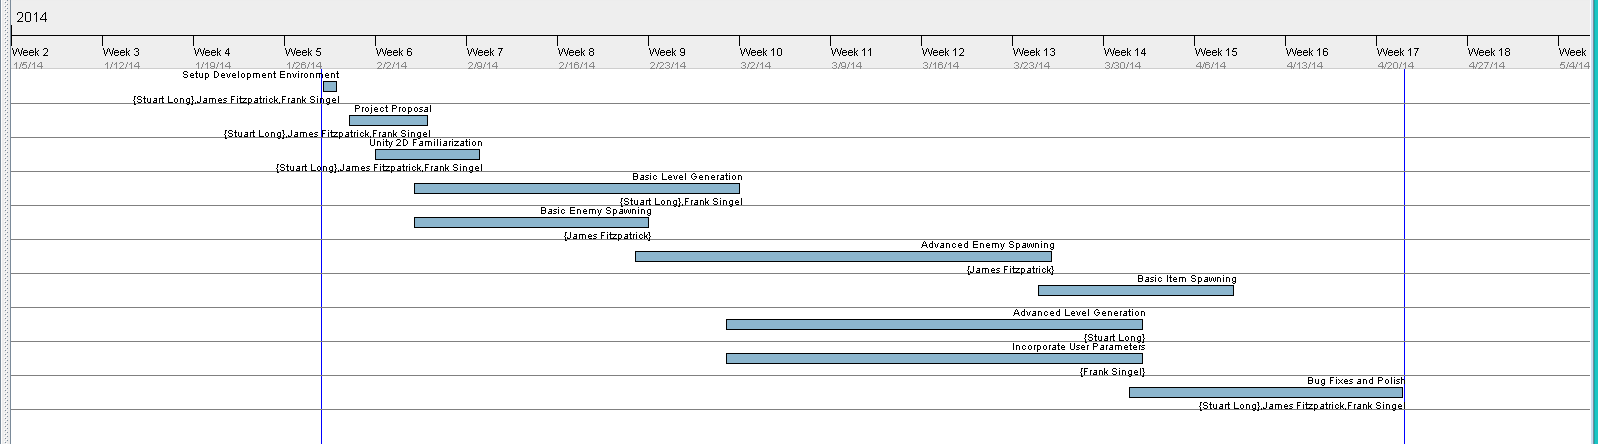
\includegraphics[width=7in]{GanttSS.png}}

\subsection{Team Responsibilities}
Below are the main responsibilities of each team member.
\begin{table}[!h]
\begin{tabularx}{\textwidth }[t]{|l|Y|}
\hline
\bfseries Team Member & \bfseries Responsibilities\\\hline
James Fitzpatrick & Any non-environmental objects including enemies and items.\\\hline
Stuart Long & Project manager and all features related to environmental objects.\\\hline
Frank Singel & Initial level generation, user parameters, and the demo game.\\\hline
\end{tabularx}
\end{table}
\subsection{Deliverables}
The final version of the project will include the \textit{Chocolate Box} library comprised of a number of scripts, documentation explaining how to use the library, and a demo game illustrating the use of the library.
\FloatBarrier
\section{User Interface}
\textit{Chocolate Box} will be fully integrated into Unity. Thus it will not requires its own User Interface. Instead, it will be used through Unity's own interface, specifically the part known as the Inspector. A mock up of this interface can be seen on the right-hand side of the figure below.\\\\
\centerline{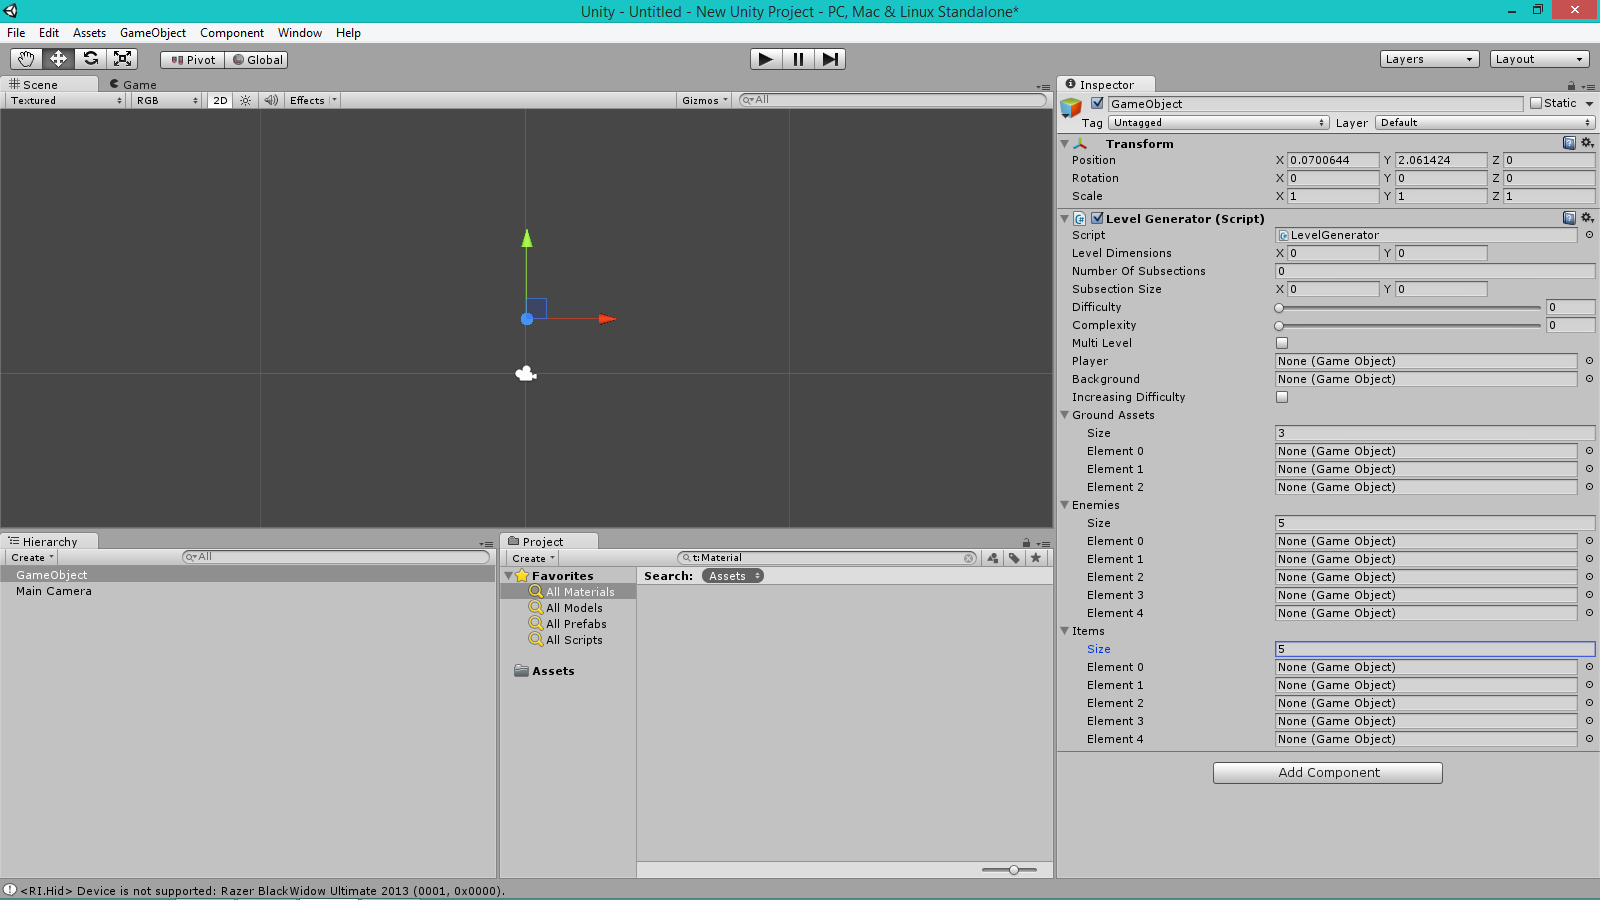
\includegraphics[width=7in]{UnitySS.png}}
\FloatBarrier
\section{Lessons Learned}
\subsection{James Fitzpatrick}
\textit{Chocolate Box} has been quite an educating experience for James. As an experienced programmer in Unity, starting the generation algorithm was as challenging as expected. However, as time rolled on, more and more external forces came into play. James has further learned of the importance of realism in goal setting. While aiming high is always a noble goal, when push comes to shove, it is important to have the important features ready and working seemless when they are needed. It is also important to remain flexible as the demands of your position may wildly change depending on the needs of the project. 

As has been a recurring theme throughout the project, being clear in communicating between subsections of the project is of great important. Small mathematical assumptions had created a cascade of unforseen consequences in erly demos. By writing clear functions rather than obscure written out calculations, you can be more sure that your code is doing what was intended by the strength of encapsulation and abstraction. 

\subsection{Stuart Long}
At the beginning of this project, Stuart already had sophisticated knowledge of both game design and Unity from his course work. Therefore the major lessons he learned throughout this project dealt with project management and developing in a team environment. As project manager, Stuart learned that, at least in the scope of a semester-long college project, tighter, more concrete deadlines result in a more efficient and effective development cycle than a more hands-off approach. Furthermore, he appreciated how effective team coding could be because this project lacked it. Because of this lack, there was occasionally confusion over certain feature or implementations. More meetings to actually discuss the code would have greatly reduced such opportunities for confusion. Stuart also gained an appreciation for how difficult it can be for several programmers to simultaneously work on a relatively small project. Even with effective version control systems, it is inevitable that they will at time get in each other's way. Finally, this project had a large focus on adapting to user input and it really showed how difficult it can be to adequately adapt to unknown and widely varying input and was the case in \textit{Chocolate Box}. More specifically, the more input and decision making you give your user, the harder your job as a developer is.
\subsection{Frank Singel}
Frank began this project with limited knowledge in the field of game design and the use of Unity, but with a knowledge of effective C\# design. As a result, Frank spent about a week just familiarizing himself with the Unity development environment. After learning effective use of Unity, he was able to begin collaborating on \textit{Chocolate Box} design in earnest. 
\section{Conclusions}
\subsection{Final Work}
The \textit{Chocolate Box} team is very proud of it's work over the semester. However, not all of the initial design goals were met. Specifically, the two main features that weren't able to be implemented were the ability to have multiple vertical sections and item generation. The reasons behind the failure to implement these two features were time constraints and other, more key features ending up being harder to implement than anticipated. Nevertheless, \textit{Chocolate Box} as it stands allow Unity developers to have infinite procedurally generated levels using their very own content and assets for their 2D platformers.
\subsection{Future Work}
While the \textit{Chocolate Box} team doesn't have any current plans to continue development on this project, the directions to be taken with it are clear. First, the two features not implemented, multiple vertical sections and item generation, would be very beneficial to users and wouldn't be that much of an extension of the current codebase. Second, this project only supports side-scrolling platformers. So, expanding \textit{Chocolate Box} to accommodate multiple different gaming genres, such as top-down shooters or puzzle games, would definitely be a great direction to go in. 
\begin{thebibliography}{3}
\bibitem{unity}Unity Technologies (2013). \textit{Unity Scripting Reference} [Online]. \url{http://docs.unity3d.com/Documentation/ScriptReference/index.html}
\end{thebibliography}

\appendix
\section{Programmer's Manual}
\subsection{Using Unity}
Unity can be installed for free from \url{https://unity3d.com/}. The Unity website also provides extensive documentation on its use.
\subsection{Chocolate Box}
\subsubsection{Installation}
\textit{Chocolate Box} is used through Unity as its own Unity project. Once completed, the source code can be obtained from \url{https://github.com/stuartlong/chocolatebox}. To open \textit{Chocolate Box} in Unity, start Unity and select "Open Project" and navigate to the /ChocolateBox/Project folder and select it.
\subsubsection{Code}
For a brief overview of the code see Section \ref{Modules}. The code itself is explained in great detail in the comments and the project documentation provided on GitHub.

\FloatBarrier
\end{document}